\section{Spiegazione del comportamento di resistori in serie ed in
	parallelo. Determinazione della resistenza equivalente.}

Si definisce \textbf{Resistenza Equivalente} di una rete di resistori la resistenza di un singolo resistore che, sottoposto alla stessa differenza di potenziale $\Delta V$ a cui \`e soggetta la rete, assorbe la stessa corrente elettrica.

Nel caso di resistori in serie avviene che:\\
\\
\noindent\begin{minipage}{0.3\textwidth}
$
\left\{
\begin{array}{lr}
	V_A - V_B = i R_1 \\	
	V_B - V_C = i R_2	\\	
	V_A - V_C = i R_{eq} \\
	V_A - V_B + V_B - V_C = V_A - V_C \\
	\\
	\textnormal{Passaggi Algebrici:}\\
	\cancel{i} R_1 + \cancel{i} R_2 = \cancel{i} R_{eq} \\
	R_1 + R_2 = R_{eq}
\end{array}
\right.
$
\end{minipage}
\hfill%
\begin{minipage}{0.6\textwidth}\raggedleft
	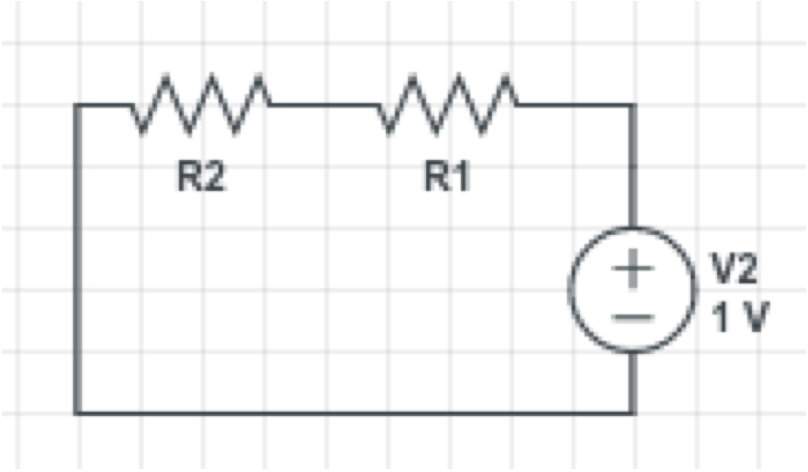
\includegraphics{serie_res}
\end{minipage}
Pertanto la $R_{eq}$ vale $R_1 + R_2$.\\
Nel caso di $n$ resistori vale la seguente formula:
\begin{equation}
    R_{eq} = \sum{R_i}
\end{equation}
Dove tutte le $R_i$ sono in serie sullo stesso ramo.\\
\noindent\begin{minipage}{0.3\textwidth}
	$
	\left\{
	\begin{array}{lr}
	V_A - V_B = i_1 R_1 \\	
	V_A - V_B = i_2 R_2	\\	
	V_A - V_B = i R_{eq} \\
	i = i_1 + i_2 \\
	\\
	\textnormal{Passaggi Algebrici:}\\
	R_{eq} = \frac{V_A - V_B}{i_1 + i_2}\\
	\frac{\cancel{V_A - V_B}}{\frac{\cancel{V_A - V_B}}{R_1} + \frac{\cancel{V_A - V_B}}{R_2}} = R_{eq}\\	
	\frac{1}{\frac{1}{R_1} + \frac{1}{R_2}} = R_{eq}\\	
	\frac{1}{R_eq} = \frac{1}{R_1} + \frac{1}{R_2}
	\end{array}
	\right.
	$
\end{minipage}
\hfill%
\begin{minipage}{0.6\textwidth}\raggedleft
	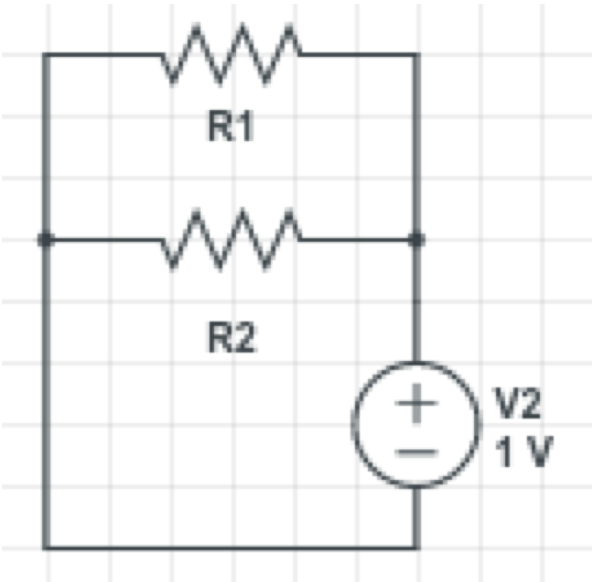
\includegraphics{parall_res}
\end{minipage}
Pertanto la $R_{eq}$ vale $\frac{1}{R_1} + \frac{1}{R_2} = \frac{R_1 + R_2}{R_1 R_2}$.\\
Nel caso di $n$ resistori vale la seguente formula:
\begin{equation}
    R_{eq} = \sum{\frac{1}{R_i}}
\end{equation}
Dove tutte le $R_i$ sono in  sullo stesso ramo.
$\hfill\square$